\chapter{Distributed Training}
\label{ch:distributed-training}

A single GPU trains a single model. A thousand GPUs do not train a thousand models---they must cooperate on one. And cooperation, in distributed systems as in human organizations, is mostly about who holds what and who talks to whom.

Chapter~\ref{ch:what-changes} ended with a verdict: a 7B model's training state needs roughly 140\,GB---more than any single GPU available today. Distributed training is not optional. But ``distributed training'' is not a single technique. It is a family of strategies, each answering a different question about what to split, what to replicate, and what price to pay in communication.

Think of it like moving a household across a city. You could rent one enormous truck (a single huge GPU---but none exists that is big enough). You could load identical copies of everything into four trucks and throw away three copies at the destination (DDP---wasteful on memory). Or you could divide your possessions across four trucks, each carrying different items, and coordinate carefully at the other end (FSDP/ZeRO). The strategies differ, but they all answer the same two questions: \emph{what goes in which truck?} and \emph{when do the trucks need to meet?}

This chapter formalizes those questions into one lens that unifies all distributed training strategies:

\begin{enumerate}[nosep]
  \item \textbf{State invariant.} What lives on which GPU? (Parameters, gradients, optimizer states, activations---each can be replicated, sharded, or recomputed.)
  \item \textbf{Flow invariant.} What data crosses GPUs at each forward, backward, and optimizer step? (AllReduce, AllGather, ReduceScatter---each has a cost proportional to the tensor size and inversely proportional to the interconnect bandwidth.)
\end{enumerate}

Every technique in this chapter---DDP, ZeRO, FSDP, tensor parallelism, pipeline parallelism, activation recomputation---is a specific answer to these two questions. The differences are not in what they compute (the math is the same single-GPU training loop from Chapter~\ref{ch:tokens-to-training}), but in \emph{where the state lives} and \emph{what flows between GPUs}. Once you internalize this lens, reading any distributed training paper or framework reduces to asking: what did they shard, and what communication did they add?

\paragraph{Running example.} We continue the thought experiment from Chapter~\ref{ch:what-changes}: training a 7B-parameter model. In Chapter~\ref{ch:what-changes}, we showed that its training state requires $\sim$140\,GB---far beyond any single GPU. Now we ask: how do you distribute that state across 4 GPUs (your Project~2 budget), 8 GPUs (a single high-end node), or 1,024 GPUs (frontier scale)? At each section, we will trace the state and flow invariants for the 7B model, making the trade-offs concrete.


\subsection*{Learning Objectives}

After completing this chapter, you should be able to:

\begin{enumerate}
  \item Explain the bandwidth hierarchy from SRAM to HBM to NVLink to InfiniBand, and state why this hierarchy determines which parallelism strategies go where.
  \item Describe AllReduce, ReduceScatter, and AllGather, and derive the communication volume for each.
  \item Trace the state and communication pattern of DDP, ZeRO-1, ZeRO-2, ZeRO-3/FSDP, and explain why they form a continuous spectrum of memory--communication trade-offs.
  \item Distinguish tensor parallelism from pipeline parallelism, and explain when each is appropriate based on interconnect bandwidth.
  \item Estimate the memory savings and compute overhead of activation recomputation.
  \item Choose a reasonable parallelism strategy for a given model size, GPU count, and interconnect, and predict its approximate memory and communication costs.
  \item Design a monitoring plan for a distributed training run: what metrics to watch, what failures to expect, and when to intervene.
\end{enumerate}


\subsection*{Notation}

\begin{center}
\begin{tabularx}{\textwidth}{@{}lX@{}}
\toprule
\textbf{Symbol} & \textbf{Meaning} \\
\midrule
$N$ & Number of model parameters \\
$G$ & Number of GPUs (``world size'') \\
$B_{\text{local}}$ & Per-GPU batch size (micro-batch size) \\
$B_{\text{global}}$ & Effective global batch size: $B_{\text{local}} \times G$ (for data parallelism) \\
$T$ & Sequence length (context window) \\
$d$ & Model dimension ($d_{\text{model}}$) \\
$L$ & Number of Transformer layers \\
$P$ & Number of pipeline stages \\
$M$ & Number of micro-batches per pipeline step \\
$\text{BW}_{\text{link}}$ & Interconnect bandwidth (bytes/second between two GPUs) \\
\bottomrule
\end{tabularx}
\end{center}


\subsection*{Timeline}

\begin{center}
\begin{tabularx}{\textwidth}{@{}lX@{}}
\toprule
\textbf{Year} & \textbf{Milestone} \\
\midrule
2012 & Krizhevsky et al. split AlexNet across two GPUs---one of the earliest uses of model parallelism in deep learning. \\
2017 & Goyal et al.~\cite{goyal2017imagenet} demonstrate linear LR scaling for large-batch distributed SGD on ImageNet. \\
2019 & Rajbhandari et al.~\cite{rajbhandari2020zero} introduce ZeRO: shard optimizer state, then gradients, then parameters across GPUs. \\
2019 & Shoeybi et al.~\cite{shoeybi2019megatron} introduce Megatron-LM: tensor parallelism for Transformer layers. \\
2020 & Narayanan et al.~\cite{narayanan2021efficient} combine tensor, pipeline, and data parallelism into 3D parallelism for trillion-parameter training. \\
2022 & PyTorch ships FullyShardedDataParallel (FSDP), a native implementation of ZeRO-3. \\
2023 & Touvron et al.~\cite{touvron2023llama} train LLaMA 65B using 3D parallelism (TP=8 within node, expert tuning of pipeline and data parallelism). \\
2024 & Jiang et al. (MegaScale)~\cite{jiang2024megascale} report automated pipeline and recovery at 10,000+ GPU scale. \\
\bottomrule
\end{tabularx}
\end{center}


%----------------------------------------------------------------------
\section{From One GPU to Many: State, Flow, and Hardware}
\label{sec:one-to-many}

\subsection{The Decision}

Chapter~\ref{ch:what-changes} did the arithmetic: a 7B model in mixed-precision training requires roughly 14\,GB for parameters (bf16), 14\,GB for gradients (bf16), 56\,GB for Adam optimizer states (fp32), and tens of GB for activations---a total well exceeding 100\,GB. No single consumer or datacenter GPU holds this. The question is not \emph{whether} to distribute, but \emph{how}.

The simplest response is to buy more identical GPUs and split the data across them (data parallelism). But this does not reduce per-GPU memory---every GPU still holds the full model. A subtler response is to split the \emph{state} itself: some GPUs hold some parameters, others hold different ones (model parallelism). The subtlest response is to split the optimizer and gradient state while keeping the model replicated for computation, then reassembling on demand (ZeRO/FSDP).

Each of these responses is a different answer to the state invariant. And each incurs a different communication pattern---the flow invariant. Before we can compare them, we need to understand the physical medium through which that communication happens.


\subsection{The Hardware Bandwidth Hierarchy}
\label{sec:bandwidth-hierarchy}

Distributed training is ultimately limited by how fast GPUs can talk to each other. The following table gives order-of-magnitude bandwidths for 2024--2026 hardware. These numbers are approximate and vary by generation, but the \emph{ratios} between tiers are remarkably stable:

\begin{center}
\begin{tabularx}{\textwidth}{@{}llXr@{}}
\toprule
\textbf{Tier} & \textbf{Link} & \textbf{Typical Use} & \textbf{Bandwidth} \\
\midrule
On-chip & SRAM $\leftrightarrow$ compute & FlashAttention tiling (\S\ref{sec:flash-attention}) & $\sim$20 TB/s \\
On-device & HBM $\leftrightarrow$ compute & Weight reads, activation writes & 2--3 TB/s \\
Intra-node & NVLink / NVSwitch & Tensor parallelism, FSDP AllGather & 600--900 GB/s \\
Inter-node & InfiniBand (IB) & Data parallelism gradient sync & 50--200 GB/s \\
Inter-node (low) & Ethernet (RoCE) & Budget clusters, inference serving & 10--50 GB/s \\
\bottomrule
\end{tabularx}
\end{center}

The key observation: \textbf{there is roughly a 10$\times$ drop at each tier}. NVLink is 10$\times$ faster than InfiniBand, which is 10$\times$ faster than commodity Ethernet. This hierarchy directly determines the design rules we will encounter throughout this chapter:

\begin{itemize}[nosep]
  \item \textbf{Communication-heavy strategies} (tensor parallelism: one AllReduce per layer per step) must stay on the fastest fabric---NVLink within a node.
  \item \textbf{Communication-light strategies} (data parallelism: one AllReduce per step for the entire gradient) can tolerate slower inter-node links.
  \item \textbf{Latency-sensitive strategies} (pipeline parallelism: many small activations between stages) prefer low-latency links.
\end{itemize}

This is the fundamental constraint. Everything that follows is an engineering response to the bandwidth hierarchy.

\begin{figure}[ht]
  \centering
  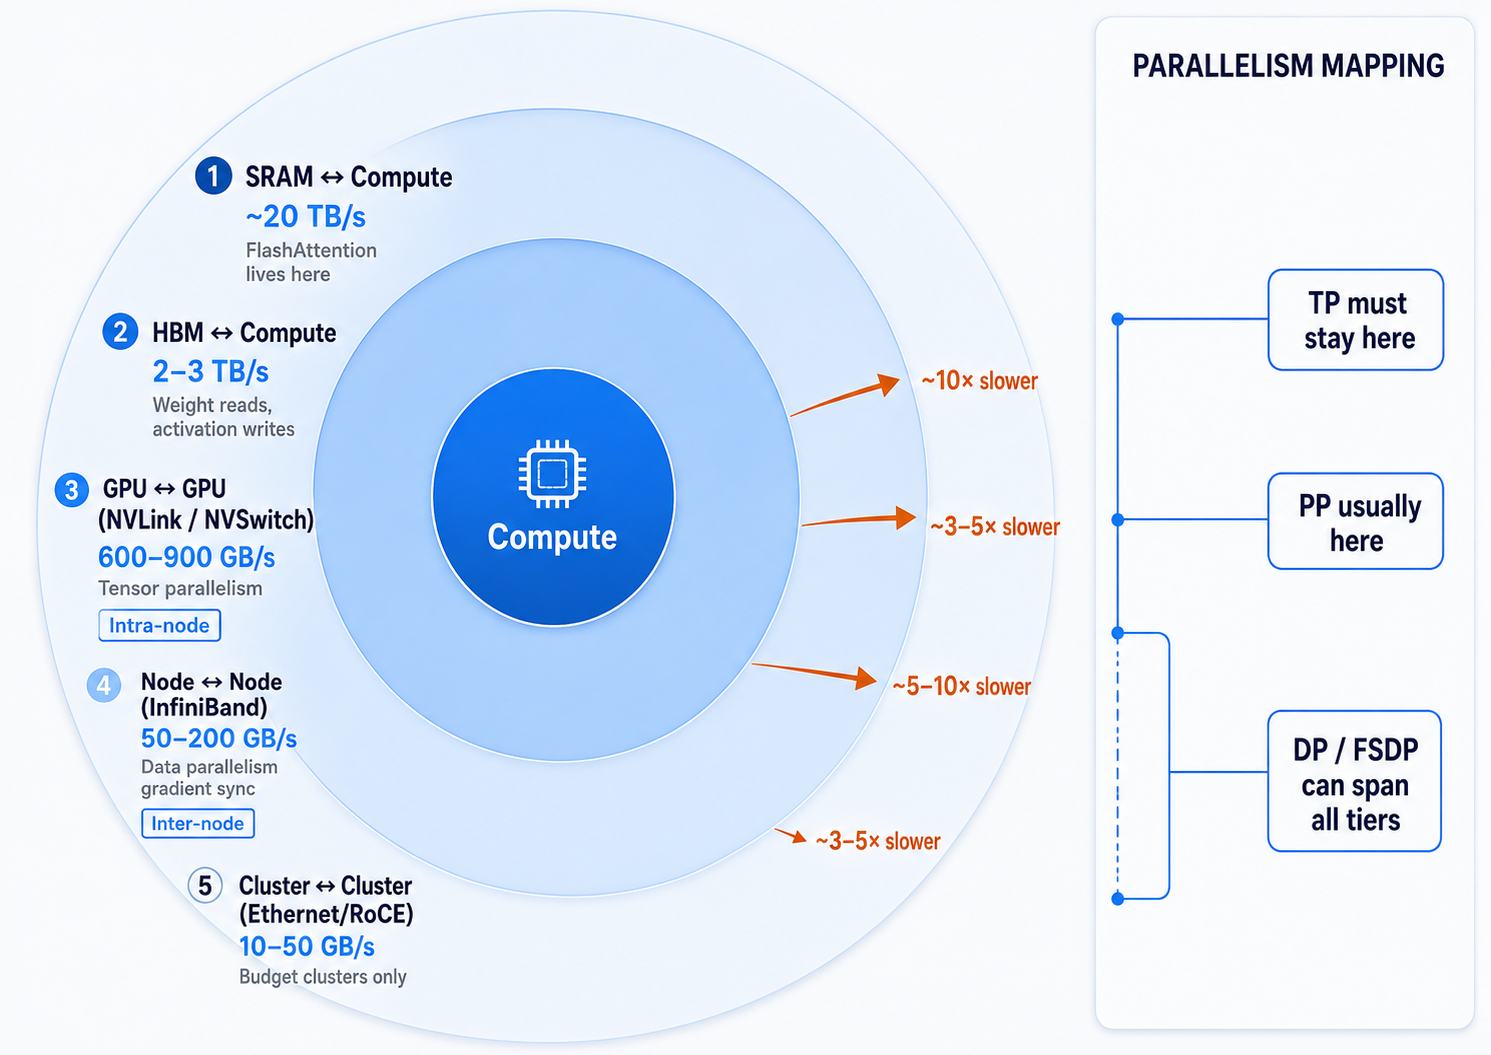
\includegraphics[width=\textwidth]{figures/ch07/fig_bandwidth_hierarchy.png}
  \caption{The bandwidth hierarchy from on-chip SRAM to cross-cluster Ethernet, with the corresponding parallelism strategies mapped to each tier. Each tier is roughly $10\times$ slower than the one inside it. Communication-heavy strategies (tensor parallelism) must stay on the fastest fabric; communication-light strategies (data parallelism) can tolerate slower links.}
  \label{fig:bandwidth-hierarchy}
\end{figure}

\paragraph{Three anchor configurations.} To keep the discussion concrete, we define three reference setups that we will return to throughout the chapter:

\begin{center}
\begin{tabularx}{\textwidth}{@{}lllX@{}}
\toprule
\textbf{Setup} & \textbf{GPUs} & \textbf{Interconnect} & \textbf{Stands For} \\
\midrule
Project~2 & 4$\times$H100 (80\,GB) & NVLink intra-node & Academic / small-team pretraining \\
Single node & 8$\times$H100 (80\,GB) & NVLink + NVSwitch & Mid-scale research lab \\
Frontier & 1024$\times$H100 & NVLink intra + IB inter & LLaMA-3, DeepSeek scale \\
\bottomrule
\end{tabularx}
\end{center}

For each technique we introduce, we will ask: does this make sense on the Project~2 setup? The single-node setup? Frontier?


\begin{quickrecap}
\textbf{Quick Recap.}
\begin{itemize}[nosep,leftmargin=1.5em]
  \item Distributed training answers two questions: what state lives on each GPU (state invariant), and what data flows between them (flow invariant).
  \item The bandwidth hierarchy (NVLink $\gg$ IB $\gg$ Ethernet) determines which strategies go where.
  \item We track three anchor configurations: 4$\times$H100 (Project~2), 8$\times$H100 (single node), and 1024$\times$H100 (frontier).
\end{itemize}
\textit{Next: the vocabulary of communication primitives that make it all work.}
\end{quickrecap}


%----------------------------------------------------------------------
\section{Communication Primitives}
\label{sec:comm-primitives}

Before we can describe any distributed training strategy, we need a shared vocabulary for how GPUs exchange data. Five collective operations underlie virtually all distributed training. We describe the three most important in detail; the other two are straightforward extensions.

\subsection{AllReduce}

AllReduce is the workhorse of data parallelism. Each of $G$ GPUs holds a tensor of the same size (e.g., the gradient $\nabla\theta$). After AllReduce, every GPU holds the \emph{sum} (or mean) of all $G$ tensors.

\paragraph{Implementation: Ring-AllReduce.} The most common implementation arranges GPUs in a logical ring. Each GPU sends a chunk to its neighbor and receives a chunk from the other direction. After $2(G-1)$ steps, every GPU has the complete sum. The total data transmitted \emph{per GPU} is:
\[
  \text{AllReduce volume per GPU} = 2 \cdot \frac{G-1}{G} \cdot |\theta| \approx 2|\theta| \quad (\text{for large } G)
\]
where $|\theta|$ is the size of the tensor in bytes. The factor of 2 comes from two phases: ReduceScatter (accumulate partial sums) and AllGather (broadcast the result).

\paragraph{Concrete example: 7B gradient sync.} Our running example has 7B parameters; gradients in bf16 occupy $7 \times 10^9 \times 2 = 14$\,GB. AllReduce on $G = 4$ GPUs moves $\approx 2 \times 14 = 28$\,GB per GPU. Over NVLink at 600\,GB/s, this takes roughly $28 / 600 \approx 0.05$ seconds. Over InfiniBand at 100\,GB/s, it would take $\sim$0.3 seconds. Over commodity Ethernet at 25\,GB/s: $\sim$1.1 seconds---which, at a step time of perhaps 2 seconds, means the GPU spends \emph{half its time waiting to communicate}. This is why the bandwidth hierarchy from \S\ref{sec:bandwidth-hierarchy} is not academic---it determines whether your training run is compute-bound or communication-bound.

\subsection{ReduceScatter and AllGather}

These are the two ``halves'' of AllReduce:

\begin{itemize}[nosep]
  \item \textbf{ReduceScatter.} Each GPU starts with the full tensor. After the operation, each GPU holds $1/G$-th of the reduced (summed) tensor. Communication volume per GPU: $\frac{G-1}{G} \cdot |\theta|$.
  \item \textbf{AllGather.} Each GPU starts with $1/G$-th of a tensor. After the operation, every GPU holds the full tensor. Communication volume per GPU: $\frac{G-1}{G} \cdot |\theta|$.
\end{itemize}

The key identity:
\[
  \boxed{\text{AllReduce} = \text{ReduceScatter} + \text{AllGather}}
\]

\begin{figure}[ht]
  \centering
  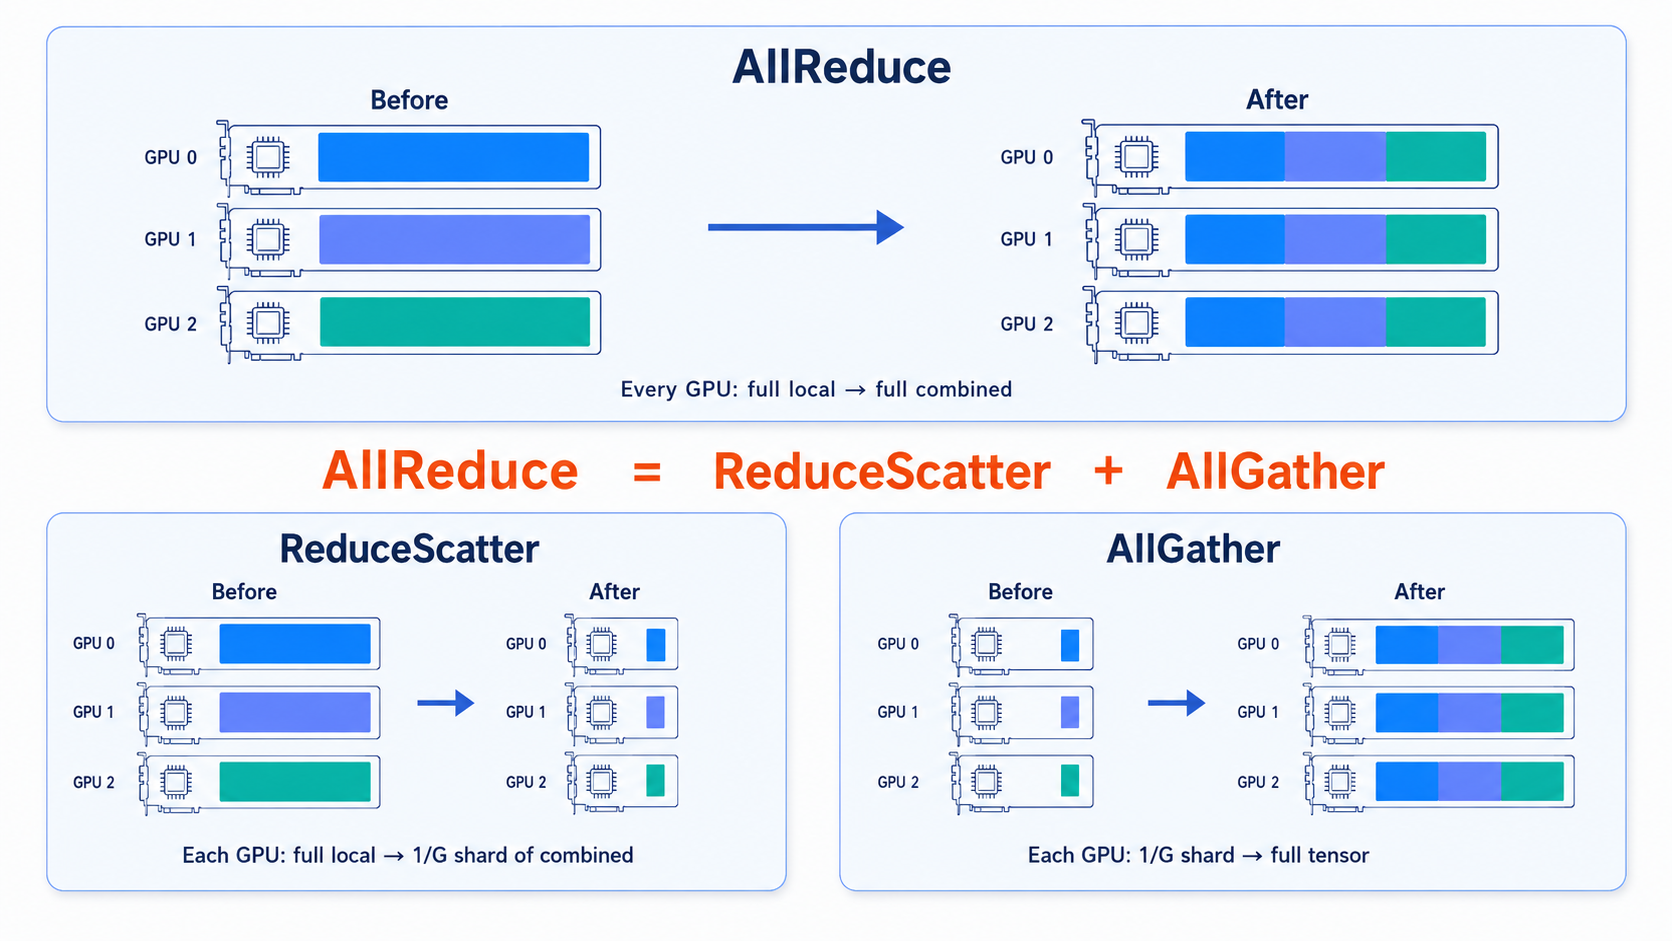
\includegraphics[width=\textwidth]{figures/ch07/fig_comm_primitives.png}
  \caption{The three core communication primitives. \textbf{AllReduce} gives every GPU the full combined result. \textbf{ReduceScatter} shrinks each GPU's tensor to a $1/G$ shard of the combined result. \textbf{AllGather} expands each GPU's shard back to the full tensor. The key identity---AllReduce $=$ ReduceScatter $+$ AllGather---is the mathematical foundation of ZeRO/FSDP.}
  \label{fig:comm-primitives}
\end{figure}

This decomposition is not just a mathematical curiosity---it is the foundation of ZeRO/FSDP. Standard DDP uses AllReduce to synchronize gradients. ZeRO-2 replaces AllReduce with ReduceScatter (each GPU keeps only its shard of the reduced gradient), saving memory at zero additional communication cost for gradients. ZeRO-3 adds an AllGather before each forward pass to reconstruct parameters on-the-fly. Understanding this decomposition is essential for understanding the DDP$\to$FSDP spectrum in \S\ref{sec:ddp-to-fsdp}.

\noindent\fbox{\parbox{\dimexpr\textwidth-2\fboxsep-2\fboxrule\relax}{\textbf{Pause and verify.} DDP uses AllReduce for gradient synchronization: each GPU sends and receives $\approx 2|\theta|$ bytes. ZeRO-2 uses only ReduceScatter: each GPU sends $\approx |\theta|$ bytes (one phase instead of two). But wait---ReduceScatter's volume per GPU is $\frac{G-1}{G} \cdot |\theta| \approx |\theta|$, which is \emph{less} than AllReduce's $2|\theta|$. Where did the savings come from? (Hint: ZeRO-2 skips the AllGather phase entirely---each GPU only needs its own $1/G$-th shard for the optimizer update, so it never reconstructs the full gradient.)}}

\subsection{Broadcast and All-to-All}

\textbf{Broadcast} sends one GPU's tensor to all others (one-to-many). \textbf{All-to-All} is a permutation: each GPU sends a different piece to each other GPU. All-to-All is less common in standard dense training but is critical for Mixture-of-Experts routing, where each token must be dispatched to its assigned expert GPU~\cite{jiang2024mixtral}. If you encounter MoE in Part~III, All-to-All is the communication primitive that makes expert routing work---and its cost is why MoE models are sensitive to load imbalance.

\begin{quickrecap}
\textbf{Quick Recap.}
\begin{itemize}[nosep,leftmargin=1.5em]
  \item AllReduce = ReduceScatter + AllGather. Total communication per GPU: $\approx 2|\theta|$.
  \item ZeRO/FSDP exploit this decomposition: ReduceScatter keeps only a shard, AllGather reconstructs on demand.
  \item All-to-All is the MoE primitive; dense training rarely uses it.
\end{itemize}
\textit{Now we have the vocabulary. Let's use it to distribute training, starting with the simplest strategy.}
\end{quickrecap}


%----------------------------------------------------------------------
\section{Data Parallelism: From DDP to FSDP}
\label{sec:ddp-to-fsdp}

This is the core section of the chapter. We present DDP, ZeRO-1, ZeRO-2, and ZeRO-3/FSDP not as four separate techniques, but as a \textbf{continuous spectrum}: at each stage, you shard one more component of the training state, trading communication for memory.

\subsection{DDP: Replicate Everything, Split the Data}

\textbf{State invariant.} Every GPU holds a complete copy of: parameters ($N$ values), gradients ($N$ values), and optimizer states (Adam~$m$ and $v$, $N$ values each). Nothing is sharded.

\textbf{Flow invariant.} Each GPU processes a different mini-batch. After the backward pass, gradients are synchronized via AllReduce so that every GPU has the same averaged gradient. Then each GPU independently runs the optimizer step.

\textbf{Memory per GPU.} Exactly the same as single-GPU training: $16N$ bytes in mixed precision (2 for bf16 params + 2 for bf16 gradients + 4+4 for fp32 Adam $m$, $v$ + 4 for fp32 master weights). For a 7B model: $\sim$112\,GB of persistent state, plus activations.

\textbf{Communication per step.} One AllReduce of the gradient tensor: $\approx 2 \times 2N$ bytes (gradients in bf16 = $2N$ bytes, AllReduce moves $\approx 2\times$ that).

\textbf{When to use it.} DDP is the right choice when the model \emph{fits} on a single GPU and you want to scale throughput by using more GPUs. For Project~1's 3.7M-parameter MiniGPT, DDP on 4 GPUs would quadruple the effective batch size with minimal overhead. But for our 7B running example, DDP alone does not help: 112\,GB does not fit on an 80\,GB GPU regardless of how many you have.

\paragraph{The batch-size coupling.} Recall from Chapter~\ref{ch:what-changes}, \S\ref{sec:pilot-runs}: when you multiply the number of GPUs by $k$ under DDP, the effective batch size also multiplies by $k$. The linear scaling rule~\cite{goyal2017imagenet} says to scale the learning rate proportionally---but this rule holds only up to a \emph{critical batch size}~\cite{mccandlish2018empirical}, beyond which $\sqrt{k}$-scaling is closer to optimal. For Project~2 (4 GPUs), linear scaling is usually fine. For frontier runs (1024 GPUs), batch-size management becomes a first-order engineering concern.


\subsection{ZeRO: Sharding the Training State}

The ZeRO optimizer~\cite{rajbhandari2020zero} observes that DDP wastes memory by replicating state that is only needed locally. The insight is surgical: \emph{keep only the shard of each state component that this GPU is responsible for updating}. The three stages of ZeRO progressively shard more:

\begin{center}
\begin{tabularx}{\textwidth}{@{}p{2cm}XXrr@{}}
\toprule
\textbf{Strategy} & \textbf{What's Sharded} & \textbf{Per-GPU Memory} & \textbf{Comm/step} & \textbf{7B (bf16)} \\
\midrule
DDP & Nothing & $16N$ & $\approx 2 \times 2N$ & 112 GB \\
ZeRO-1 & Optimizer states & $4N + 12N/G$ & $\approx 2 \times 2N$ & 37 GB ($G\!=\!4$) \\
ZeRO-2 & + Gradients & $4N + 14N/G$ & $\approx 2 \times 2N$ & 31 GB ($G\!=\!4$) \\
ZeRO-3 & + Parameters & $16N/G$ & $\approx 3 \times 2N$\textsuperscript{*} & 28 GB ($G\!=\!4$) \\
\bottomrule
\end{tabularx}
\end{center}

\noindent In the communication column, $2N$ means the byte size of one bf16 model-sized tensor: $N$ parameters $\times$ 2 bytes. Thus $2 \times 2N$ is the approximate per-GPU traffic of one model-sized AllReduce, and $3 \times 2N$ is 1.5$\times$ DDP's volume---only 50\% more bytes, despite sharding everything.

\noindent\textit{\textsuperscript{*}ZeRO-3 adds an AllGather of parameters before each forward/backward layer, costing an additional $\sim 2N$ bytes of communication per step beyond the $2 \times 2N$ of AllReduce-equivalent gradient sync. The exact overhead depends on whether communication overlaps with computation.}

\begin{figure}[ht]
  \centering
  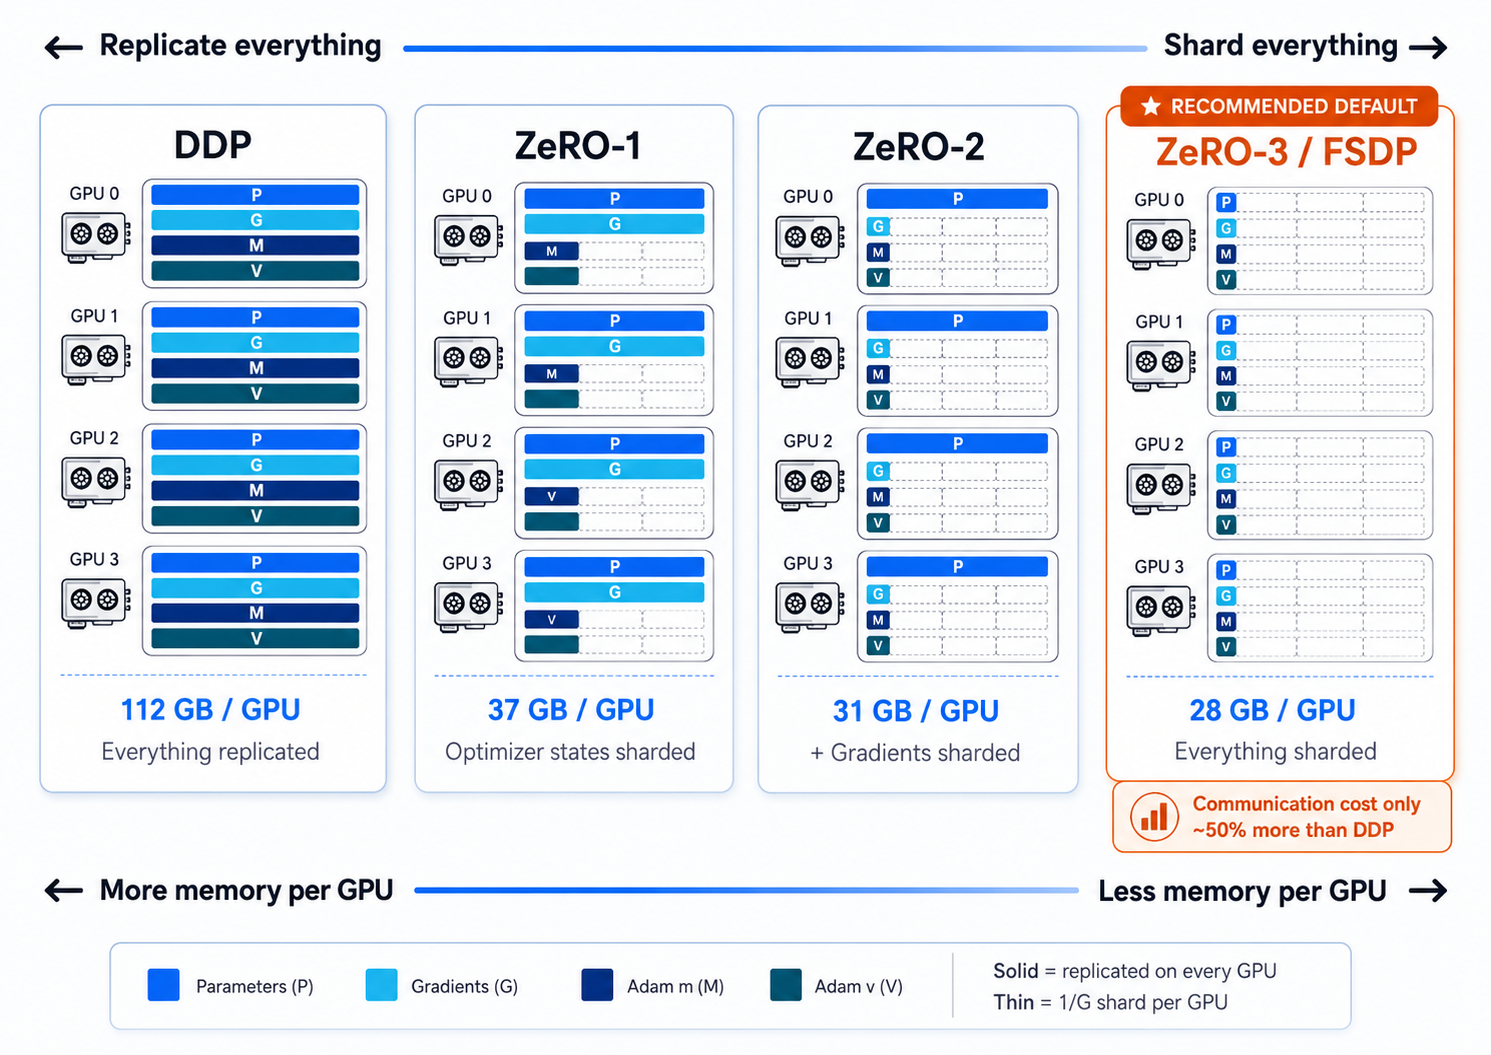
\includegraphics[width=\textwidth]{figures/ch07/fig_ddp_to_fsdp.png}
  \caption{The DDP-to-FSDP spectrum: from ``replicate everything'' to ``shard everything.'' Each card shows 4~GPUs and their training state. In DDP, every GPU holds a full copy (112\,GB). ZeRO-1 shards optimizer states (37\,GB). ZeRO-2 adds gradient sharding (31\,GB). ZeRO-3/FSDP shards all state (28\,GB per GPU)---the recommended default for Project~2.}
  \label{fig:ddp-to-fsdp}
\end{figure}

\paragraph{Reading the table.} Follow the 7B column from top to bottom. DDP requires 112\,GB per GPU---impossible on an 80\,GB H100. ZeRO-1 drops to 37\,GB per GPU (with $G=4$) by sharding the 56\,GB of Adam states across 4 GPUs. ZeRO-2 shards gradients too, reaching 31\,GB. ZeRO-3 shards everything: 28\,GB per GPU, comfortably within an 80\,GB card---leaving $\sim$50\,GB for activations.

\paragraph{The key insight.} ZeRO-2's gradient synchronization uses ReduceScatter instead of AllReduce---each GPU keeps only its $1/G$-th shard of the summed gradient. The total communication volume is the same as DDP's AllReduce (recall: AllReduce = ReduceScatter + AllGather). ZeRO-2 simply \emph{stops before the AllGather step}, since each GPU only needs its own shard for the optimizer update. \textbf{You get memory savings at no additional communication cost.}

ZeRO-3 goes further: parameters are also sharded, so before each forward or backward pass through a layer, the GPU must AllGather the full parameters for that layer from all other GPUs. This adds communication---but the transfer can overlap with computation on the previous layer, hiding much of the cost in practice.

\paragraph{The surprising trade-off.} A common misconception is that more sharding means dramatically more communication. In reality, the total communication \emph{volume} of ZeRO-3/FSDP is about 1.5$\times$ DDP's: DDP moves $\sim\!2|\theta|$ bytes (one AllReduce), while ZeRO-3 moves $\sim\!3|\theta|$ bytes (ReduceScatter for gradients + AllGather for parameters in forward + AllGather for parameters in backward). But these transfers overlap with computation---the AllGather for layer $\ell+1$ can prefetch while layer $\ell$ is computing---so the measured \emph{wall-clock} overhead is often well under 50\%. Meanwhile, the memory savings are $G\times$---a factor of 4 on our Project~2 setup. \textbf{A mild increase in communication volume buys a 4$\times$ reduction in per-GPU memory.} This is why FSDP is almost always worth it.

\noindent\fbox{\parbox{\dimexpr\textwidth-2\fboxsep-2\fboxrule\relax}{\textbf{Pause and verify.} Using the table above, compute the per-GPU memory for a 300M-parameter model (Project~2's target) under DDP and FSDP (ZeRO-3) with $G = 4$ GPUs. Under DDP, does the model fit on an H100 (80\,GB)? Under FSDP? How much memory is left for activations in each case?}}


\subsection{PyTorch FSDP}

PyTorch's FullyShardedDataParallel (FSDP) is the native implementation of ZeRO-3. In practice, using FSDP involves three decisions:

\begin{enumerate}[nosep]
  \item \textbf{Wrapping policy.} Which modules to shard. Typically, each Transformer block is wrapped as one FSDP unit. Wrapping too finely increases communication overhead; wrapping too coarsely limits memory savings.
  \item \textbf{Sharding strategy.} FSDP supports full shard (ZeRO-3), shard grad+optimizer (ZeRO-2), and no shard (DDP). Hybrid strategies---ZeRO-3 within a node, ZeRO-1 across nodes---balance memory savings against cross-node communication cost.
  \item \textbf{Mixed precision.} FSDP can keep parameters in bf16 for computation and fp32 for optimizer updates, matching the mixed-precision recipe from Chapter~\ref{ch:tokens-to-training}.
\end{enumerate}

For Project~2 (4$\times$H100 on a single node with NVLink), full FSDP sharding is the recommended default. The AllGather communication for parameter reconstruction is fast over NVLink ($\sim$600\,GB/s), and the memory savings are substantial.


\begin{quickrecap}
\textbf{Quick Recap.}
\begin{itemize}[nosep,leftmargin=1.5em]
  \item DDP replicates everything and synchronizes gradients via AllReduce. It does not save per-GPU memory.
  \item ZeRO-1/2/3 progressively shard optimizer states, gradients, and parameters. Each stage trades communication for memory.
  \item FSDP (ZeRO-3) is the PyTorch default for models that don't fit on one GPU. It shards all training state and reconstructs parameters on-the-fly via AllGather.
  \item ZeRO-2 saves memory \emph{at no additional communication cost} over DDP---it simply stops the AllGather phase for gradients.
\end{itemize}
\textit{DDP and FSDP distribute the training state. But what about the computation itself?}
\end{quickrecap}


%----------------------------------------------------------------------
\section{Model Parallelism: Tensor and Pipeline}
\label{sec:model-parallelism}

FSDP shards persistent state, but each layer's forward pass still requires assembling the full layer's parameters and computing on the full per-rank batch. For models in the 70B+ range, even one layer's worth of activations and parameter materialization can exceed a single GPU. And for very long sequences ($T \geq 8192$), per-layer activation tensors dominate memory regardless of model size. Model parallelism addresses these cases by splitting the \emph{computation itself} across GPUs, not just the state. Two complementary strategies exist.

\subsection{Tensor Parallelism}
\label{sec:tensor-parallelism}

\textbf{Idea.} Split each layer's weight matrices across GPUs. Each GPU computes a partial result; the partials are combined via AllReduce.

\textbf{For the FFN block:} The first linear projection $W_1 \in \mathbb{R}^{d \times 4d}$ is split by columns across $G$ GPUs---each GPU holds $W_1^{(g)} \in \mathbb{R}^{d \times 4d/G}$ and computes $Y^{(g)} = XW_1^{(g)}$. The activation function is applied independently. The second projection $W_2 \in \mathbb{R}^{4d \times d}$ is split by rows; each GPU computes $Z^{(g)} = Y^{(g)} W_2^{(g)}$. The final output is an AllReduce (sum) of the $Z^{(g)}$.

\textbf{For the attention block:} Each GPU gets a subset of attention heads. Since heads are independent, this is a natural split. The output projection then requires an AllReduce.

\textbf{State invariant.} Each GPU holds $1/G$-th of each layer's parameters. Activations are split correspondingly.

\textbf{Flow invariant.} Two AllReduce operations per Transformer block (one for attention output, one for FFN output). This is \emph{per layer, per step}---far more frequent than DDP's single AllReduce per step.

\textbf{Communication cost.} For a model with $L$ layers, each forward+backward pass requires $4L$ AllReduce operations (2 forward + 2 backward per block). Each AllReduce communicates an activation tensor of shape $B_{\text{local}} \times T \times d$, not just a batch of hidden vectors. Here $B_{\text{local}}$ means the per-TP-group micro-batch size for one forward+backward micro-step; if you use gradient accumulation, multiply the total traffic by the number of accumulated micro-steps. In bf16, the tensor size is $B_{\text{local}} \cdot T \cdot d \cdot 2$ bytes; a ring AllReduce moves roughly twice that amount per GPU.

For our 7B running example ($d = 4096$, $B_{\text{local}} = 4$, $T = 2048$, $L = 32$): each activation tensor for one micro-step is
\[
  4 \times 2048 \times 4096 \times 2 \approx 67\,\text{MB}.
\]
A ring AllReduce moves roughly $2 \times 67 \approx 134$\,MB per GPU. With $4 \times 32 = 128$ AllReduce operations per forward+backward micro-step, tensor parallelism moves on the order of $17$\,GB per GPU. On NVLink at 600\,GB/s, the bandwidth cost alone is roughly $17/600 \approx 28$\,ms, before accounting for latency and imperfect overlap. On InfiniBand, the same traffic is much more expensive. The lesson is the same, but stronger: TP is not just frequent communication; it is frequent communication of sequence-length-sized activation tensors.

\paragraph{Design rule.} \emph{Tensor parallelism stays within a node.} The per-layer AllReduce frequency demands the highest available bandwidth---NVLink, not InfiniBand. This is why Megatron-LM~\cite{shoeybi2019megatron} and LLaMA use TP$=$8 (matching the 8 GPUs within a DGX node) and never TP across nodes.

\paragraph{Project~2 (4$\times$H100).} TP is optional. FSDP alone provides sufficient memory savings for a 300M--1B model. TP would help if you want to maximize batch size, but it adds engineering complexity. Our recommendation: start with pure FSDP and only add TP if memory profiling shows you need it.


\subsection{Pipeline Parallelism}
\label{sec:pipeline-parallelism}

\textbf{Idea.} Assign different groups of layers to different GPUs. GPU~0 runs layers 1--8, GPU~1 runs layers 9--16, and so on. Each GPU only holds $L/P$ layers (where $P$ is the number of pipeline stages).

\textbf{State invariant.} Each GPU holds a contiguous subset of the model's layers---all their parameters, gradients, and optimizer states.

\textbf{Flow invariant.} Between stages, the activation tensor (shape $B \times T \times d$) is transmitted from one GPU to the next. This is a point-to-point send, not a collective---and it happens $P-1$ times per forward pass.

\textbf{The bubble problem.} Consider 4 pipeline stages processing a single micro-batch. GPU~0 computes forward for layers 1--8 and sends the activation to GPU~1. While GPU~1 computes, GPU~0 is idle. While GPU~3 computes, GPUs~0--2 are idle. The backward pass has the same issue in reverse. For a single micro-batch, GPU utilization is approximately $1/P$---75\% wasted with 4 stages.

\textbf{Micro-batching.} The standard mitigation: split the mini-batch into $M$ micro-batches and pipeline them. GPU~0 starts the forward pass on micro-batch 2 while GPU~1 processes micro-batch 1. The bubble fraction becomes approximately $(P-1) / (P-1 + M)$. With $M = 16$ and $P = 4$: bubble $\approx$ 16\%---much better than 75\%, but still non-trivial.

\paragraph{1F1B scheduling.} The ``one-forward-one-backward'' schedule interleaves forward and backward micro-batches to reduce peak memory. Instead of running all $M$ forwards then all $M$ backwards (which stores $M$ activations simultaneously), 1F1B ensures that, in steady state, each pipeline stage alternates between one forward and one backward. This limits peak activation memory to roughly $P$ micro-batches instead of $M$---a significant saving when $M \gg P$.

\paragraph{When to use pipeline parallelism.} PP is most useful when you have \emph{many nodes} connected by inter-node links. The activation tensors transmitted between stages are relatively small ($B \times T \times d$ per micro-batch), so PP tolerates InfiniBand latency better than TP's per-layer AllReduce. PP also doesn't require modifying the layer's internal computation---you can pipeline any model whose layers are sequential.

\begin{figure}[ht]
  \centering
  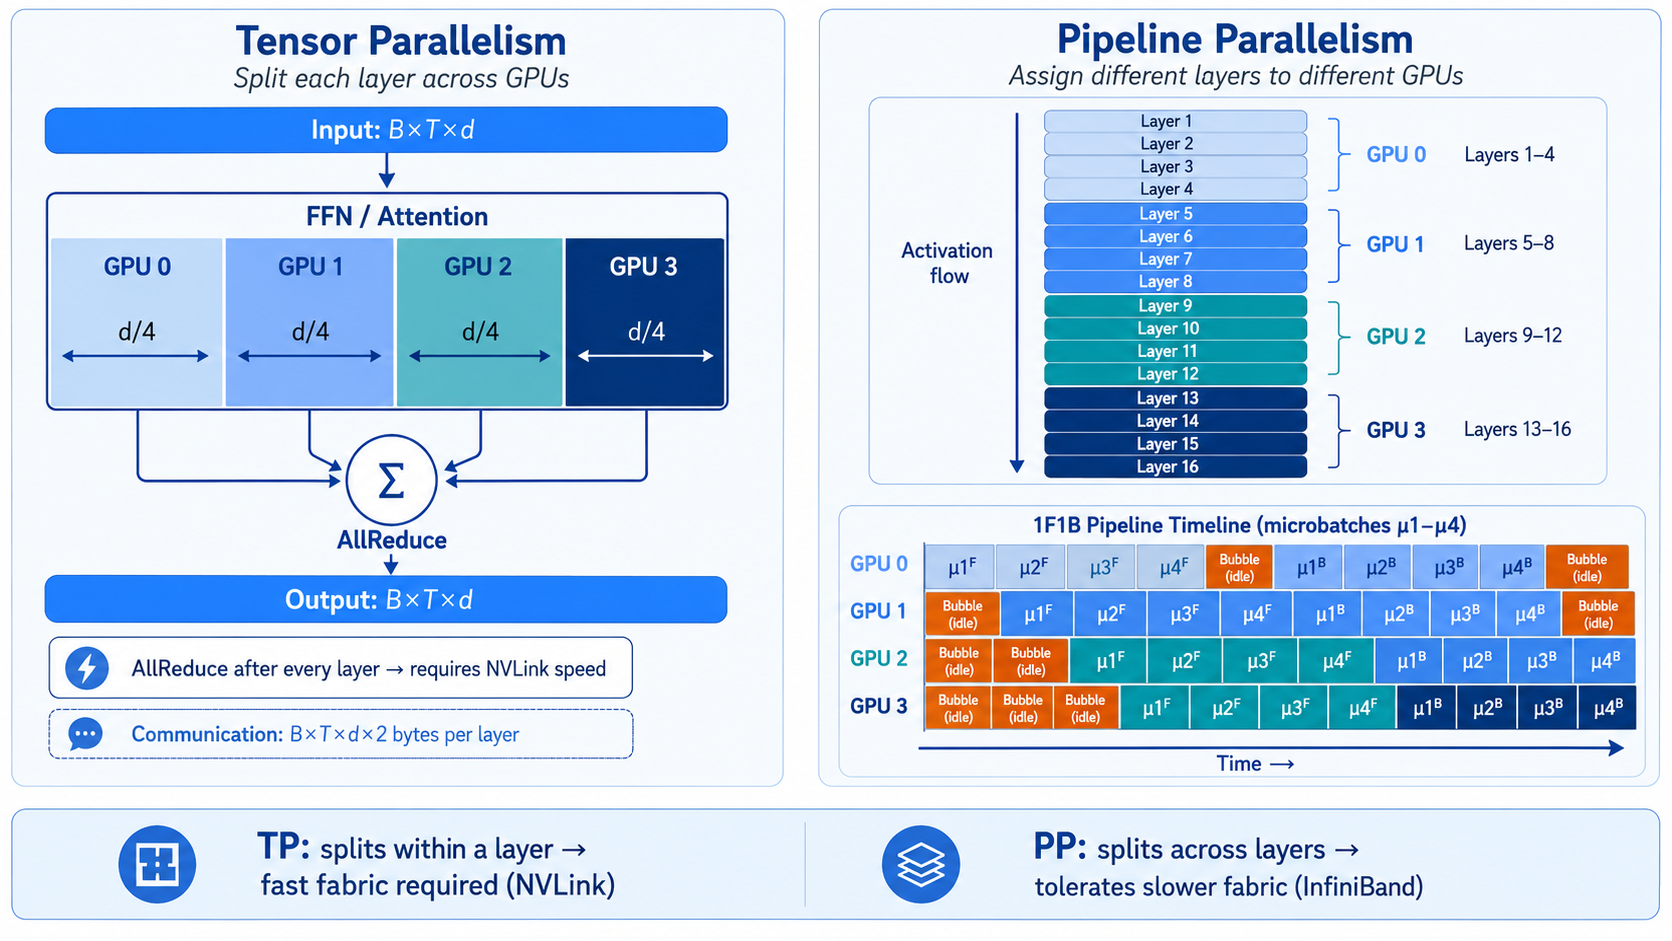
\includegraphics[width=\textwidth]{figures/ch07/fig_tp_pp.png}
  \caption{\textbf{Left:} Tensor parallelism splits each layer's weight matrices across GPUs. Each GPU computes a partial result; partials are combined via AllReduce after every layer. \textbf{Right:} Pipeline parallelism assigns layer groups to different GPUs. The 1F1B (one-forward-one-backward) schedule interleaves micro-batches to reduce the pipeline bubble (shown in orange), but idle time remains.}
  \label{fig:tp-pp}
\end{figure}

\paragraph{Project~2 (4$\times$H100).} PP is not recommended. With only 4 GPUs on a single NVLink node, the pipeline bubble overhead is significant, and FSDP provides sufficient memory savings without introducing the complexity of micro-batch scheduling and inter-stage communication.


\begin{quickrecap}
\textbf{Quick Recap.}
\begin{itemize}[nosep,leftmargin=1.5em]
  \item Tensor parallelism splits each layer's weights; it requires AllReduce per layer and demands NVLink-class bandwidth.
  \item Pipeline parallelism assigns layer groups to different GPUs; it tolerates slower links but suffers pipeline bubbles.
  \item Design rule: TP within nodes (fast links), PP across nodes (tolerates slower links), DP/FSDP everywhere.
  \item Project~2 should use FSDP, not TP or PP.
\end{itemize}
\textit{Model parallelism addresses the model's computation. But activations can still dominate memory---especially with long sequences and large batches. Next: trading compute to reclaim that memory.}
\end{quickrecap}


%----------------------------------------------------------------------
\section{Activation Recomputation}
\label{sec:activation-recomputation}

FSDP solved the persistent-state problem: our 7B model's parameters, gradients, and optimizer fit in 28\,GB per GPU (with $G = 4$). But during the forward pass, each layer produces intermediate activations that must be stored for the backward pass. For 7B ($L = 32$, $d = 4096$, $T = 2048$, $B_{\text{local}} = 4$, bf16), the activation memory is roughly $B \times T \times d \times L \times c \approx 4 \times 2048 \times 4096 \times 32 \times 10 \approx 10$\,GB per GPU. That fits alongside the 28\,GB of sharded state---but only barely. Increase the batch size to 16 or the context to 4096, and activations alone blow past 40\,GB.

\textbf{Activation recomputation} (also called \emph{gradient checkpointing}) trades compute for memory: instead of storing all intermediate activations, it discards them after the forward pass and \emph{recomputes} them during the backward pass. The memory savings are dramatic; the compute cost is one additional forward pass.

\subsection{Full Recomputation}

Store only the input to each Transformer block. During backward, rerun the forward pass for each block to regenerate its activations. Memory: $O(B \cdot T \cdot d)$ per checkpoint (down from $O(B \cdot T \cdot d \cdot L)$ for all layers). Compute overhead: up to $\sim$33\% in the full-recomputation case (one additional forward pass, which is roughly 1/3 of the forward+backward total). In practice, this is an upper bound---selective recomputation (\S\ref{sec:selective-recompute}) and FlashAttention's built-in recomputation reduce the actual overhead to 5--15\%.

\subsection{Selective Recomputation}
\label{sec:selective-recompute}

Not all operations cost the same. Attention's QKV projections and FFN linear layers are expensive (matrix multiplies), while LayerNorm and dropout are cheap. Selective recomputation~\cite{korthikanti2023reducing} stores the outputs of expensive operations and recomputes only the cheap ones. This reduces the compute overhead to $\sim$5\%--10\% while still saving most of the activation memory.

\paragraph{Interaction with FlashAttention.} FlashAttention (Chapter~\ref{ch:what-changes}, \S\ref{sec:flash-attention}) already avoids materializing the $T \times T$ attention matrix---effectively recomputing it during backward. When both FlashAttention and activation recomputation are enabled, the combined memory savings are multiplicative: FlashAttention eliminates the $O(T^2)$ attention matrix, and recomputation eliminates the $O(L)$ layer-wise activation storage.

\paragraph{Project~2.} For training a 300M--1B model on 4$\times$H100 with FSDP, activation recomputation is often needed when using long contexts ($T = 2048$+) or large batch sizes. Enabling it in PyTorch is one line: \texttt{torch.utils.checkpoint.checkpoint(block, input)}.

\noindent\fbox{\parbox{\dimexpr\textwidth-2\fboxsep-2\fboxrule\relax}{\textbf{Pause and verify.} A 300M model with 24 layers, $d = 1024$, $T = 2048$, and $B_{\text{local}} = 8$ (bf16). Estimate the activation memory without recomputation: $B \times T \times d \times L \times c$ bytes with $c \approx 10$. Now estimate with full recomputation (only one block's activations stored at a time). How much memory does recomputation save? What is the approximate compute overhead?}}


%----------------------------------------------------------------------
\section{3D Parallelism in Practice}
\label{sec:3d-parallelism}

Real frontier training runs combine multiple parallelism strategies. The standard combination is called \textbf{3D parallelism}: Tensor Parallelism (TP) $\times$ Pipeline Parallelism (PP) $\times$ Data Parallelism (DP/FSDP), forming a three-dimensional grid of GPUs.

\subsection{The Design Rule}

The allocation follows the bandwidth hierarchy from \S\ref{sec:bandwidth-hierarchy}:

\begin{enumerate}[nosep]
  \item \textbf{Innermost (fastest link):} TP within a node. Typically TP$=$8 on an 8-GPU DGX/HGX node.
  \item \textbf{Middle:} PP across a few adjacent nodes. Activation tensors between pipeline stages are small enough for inter-node IB.
  \item \textbf{Outermost (slowest link):} DP/FSDP across all remaining GPUs. Gradient synchronization is one AllReduce per step---amortized over many layers of computation.
\end{enumerate}

\paragraph{Example: frontier 7B on 256 GPUs (32 nodes $\times$ 8 GPUs).}

\begin{center}
\begin{tabular}{@{}llll@{}}
\toprule
\textbf{Dimension} & \textbf{Size} & \textbf{Where} & \textbf{Communication} \\
\midrule
TP & 8 & intra-node (NVLink) & AllReduce per layer \\
PP & 1 & --- & (not needed at 7B) \\
DP/FSDP & 32 & inter-node (IB) & AllReduce per step \\
\bottomrule
\end{tabular}
\end{center}

For a 70B model on 1024 GPUs, a typical configuration might be TP=8, PP=8, DP=16. The exact configuration depends on the model's layer count, per-layer memory, and the cluster's interconnect topology.

\paragraph{Walking the state and flow.} The 3D configuration is where the two invariants pay off. Consider the 70B example with TP=8, PP=8, and DP=16:

\begin{itemize}[nosep,leftmargin=1.5em]
  \item \textbf{State placement.} Each TP group holds one shard of a layer's matrices. Each PP stage owns a contiguous slice of the layer stack. Each DP group owns a replica of the whole pipeline, usually with ZeRO/FSDP sharding applied inside the DP dimension to avoid replicating optimizer state.
  \item \textbf{Forward flow.} Within a layer, TP GPUs exchange partial activations through fast intra-node AllReduce. Between pipeline stages, activations move point-to-point from one stage to the next. Across DP replicas, there is no forward communication for ordinary dense models.
  \item \textbf{Backward flow.} The same paths run in reverse: pipeline stages send activation gradients backward, TP groups AllReduce partial gradients inside each layer, and the DP/FSDP dimension ReduceScatters gradients so each rank updates only its shard.
  \item \textbf{Why the placement works.} The highest-frequency communication (TP) stays on NVLink. Medium-frequency point-to-point activation traffic (PP) can cross nodes. Lowest-frequency synchronization (DP/FSDP) spans the full cluster. The parallelism strategy is not arbitrary; it is the bandwidth hierarchy written into the training graph.
\end{itemize}

\begin{figure}[ht]
  \centering
  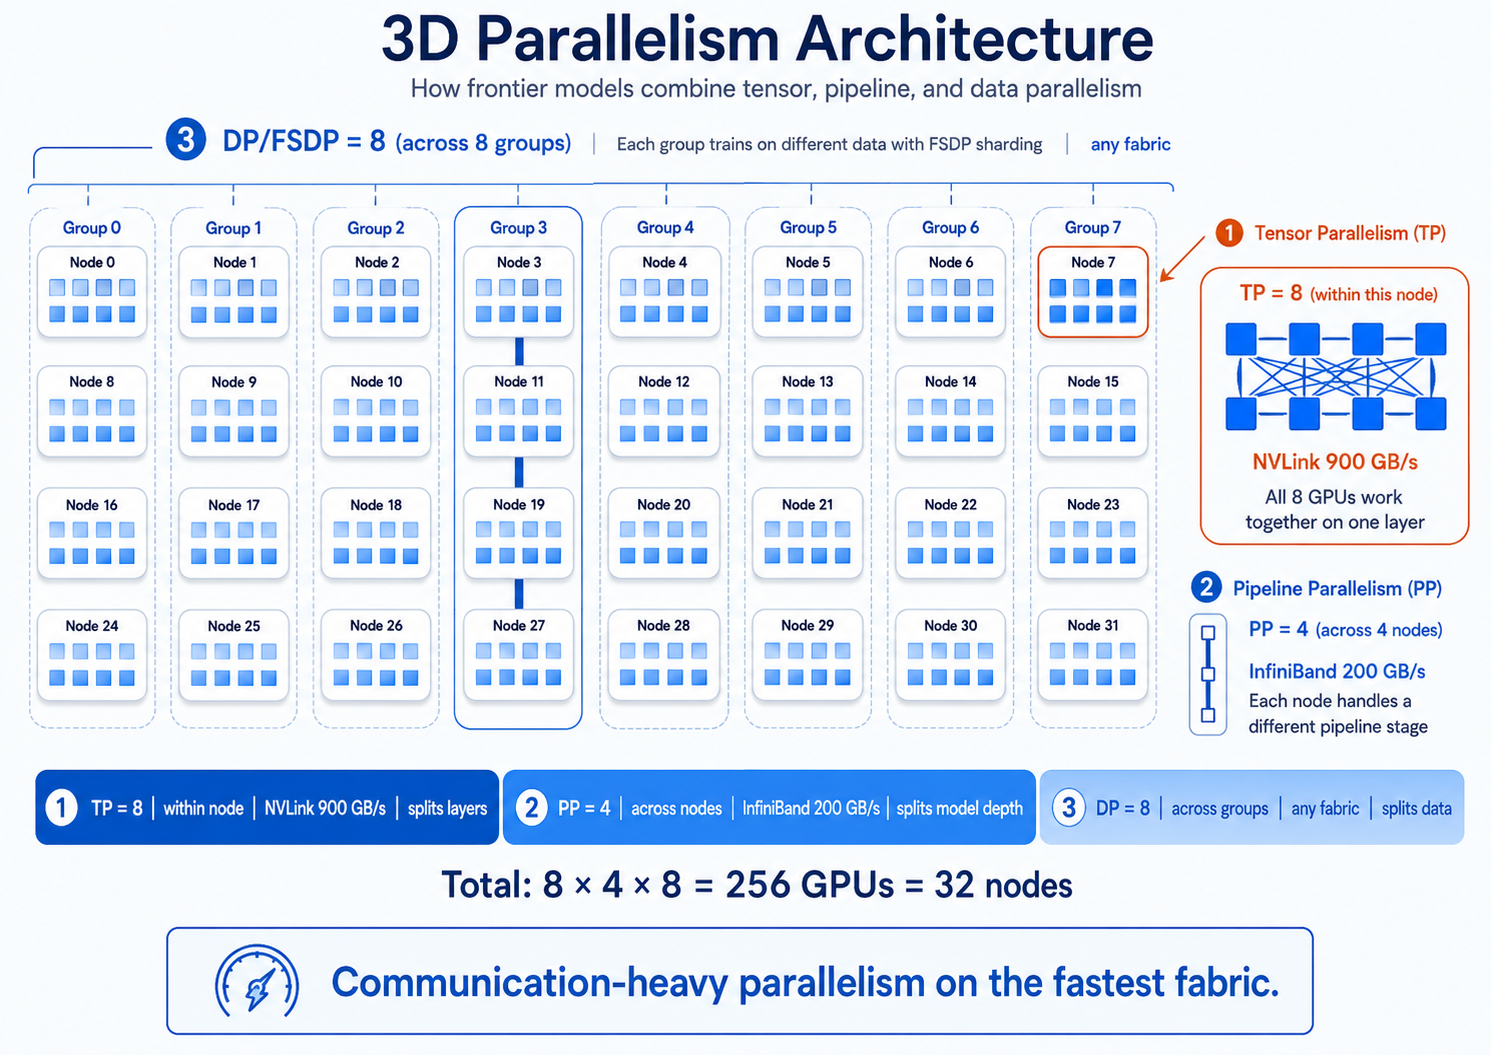
\includegraphics[width=\textwidth]{figures/ch07/fig_3d_parallelism.png}
  \caption{3D parallelism at frontier scale. Tensor parallelism (TP$=$8) stays within a node on NVLink. Pipeline parallelism (PP$=$4) spans across a small group of nodes. Data parallelism (DP$=$8) replicates across all groups. The design rule: communication-heavy parallelism on the fastest fabric.}
  \label{fig:3d-parallelism}
\end{figure}

\paragraph{FSDP as a fourth dimension.} In practice, many teams use FSDP within the DP dimension: each DP rank further shards its optimizer states via ZeRO-1 or ZeRO-2. This gives ``3.5D'' parallelism: TP $\times$ PP $\times$ DP $\times$ FSDP-sharding. The terminology varies; the principle is consistent---shard everything you can, communicate only what you must.

\subsection{MoE Parallelism}

Mixture-of-Experts models (Chapter~\ref{ch:what-changes}, \S\ref{sec:frontier-variants}) add a fourth parallelism dimension: \textbf{expert parallelism}. Each expert lives on a specific GPU. During the forward pass, tokens are routed to their assigned expert via All-to-All communication. This creates a communication pattern distinct from AllReduce: the traffic is data-dependent (it depends on the router's decisions), and load imbalance across experts translates directly into GPU idle time. MoE's engineering challenges---load-balancing losses, dropped tokens, capacity factors---are beyond the scope of this chapter but represent an active area of systems research.


%----------------------------------------------------------------------
\section{Throughput and MFU}
\label{sec:throughput-mfu}

Distributed training is only useful if the GPUs are actually doing productive work. Two metrics quantify this.

\subsection{Tokens per Second per GPU}

The most intuitive throughput metric:
\[
  \text{Throughput} = \frac{B_{\text{global}} \times T}{\text{step time} \times G} \quad [\text{tokens/sec/GPU}]
\]

This number is easy to compute and easy to compare across setups. A typical H100 achieves 3,000--10,000 tokens/sec/GPU for a 7B model, depending on batch size, sequence length, and parallelism strategy.

\subsection{Model FLOPS Utilization (MFU)}

MFU measures what fraction of the GPU's theoretical peak compute you are actually using:
\[
  \text{MFU} = \frac{\text{model FLOPs per step / step time}}{\text{GPU peak FLOPS (bf16)}}
\]

\textbf{Model FLOPs} counts only the ``useful'' floating-point operations (forward + backward through the model), excluding communication, data loading, and framework overhead. For a Transformer, the model FLOPs per step are approximately $6 \times N \times B_{\text{global}} \times T$ (2 for forward, 4 for backward with recomputation).

Typical MFU values:
\begin{itemize}[nosep]
  \item \textbf{40--55\%}: Good single-node training with FSDP.
  \item \textbf{30--45\%}: Multi-node training with some communication overhead.
  \item \textbf{$<$30\%}: Likely a bottleneck---investigate data loading, communication, or Python overhead.
\end{itemize}

\paragraph{Bottleneck diagnosis.} When MFU is low, check these in order:
\begin{enumerate}[nosep]
  \item \textbf{Data loading.} Is the GPU waiting for data? Use \texttt{num\_workers > 0} in DataLoader.
  \item \textbf{Communication.} Is AllReduce / AllGather taking too long? Profile with \texttt{NCCL\_DEBUG=INFO} or PyTorch profiler.
  \item \textbf{Memory thrashing.} Is the GPU near its memory limit, causing frequent cache evictions? Reduce batch size or enable activation recomputation.
  \item \textbf{Uneven load.} In pipeline parallelism, are some stages slower than others? Check per-GPU step times.
  \item \textbf{Python overhead.} For small models with fast steps, Python's GIL and framework overhead can dominate. Compile with \texttt{torch.compile} if applicable.
\end{enumerate}

\noindent\fbox{\parbox{\dimexpr\textwidth-2\fboxsep-2\fboxrule\relax}{\textbf{Pause and verify.} Compute the MFU for our 7B running example on 4$\times$H100. Assume: $B_{\text{global}} = 32$, $T = 2048$, step time $= 2.5$ seconds. Model FLOPs per step $\approx 6 \times 7 \times 10^9 \times 32 \times 2048 \approx 2.75 \times 10^{15}$. Each H100 has $\sim$990 TFLOPS (bf16 peak). Total peak for 4 GPUs $= 3.96 \times 10^{15}$ FLOPS/sec. MFU $= (2.75 \times 10^{15} / 2.5) / (3.96 \times 10^{15}) \approx 28\%$. Is this realistic? (Hint: reverse-derive the step time. At 50\% MFU, the sustained compute is $\sim$2 PFLOPS, so processing 2.75 PFLOP should take $\sim$1.4 seconds of pure compute---the remaining 1.1 seconds is communication and overhead. A 28\% MFU on 4 H100s suggests a significant bottleneck. Check data loading, FSDP AllGather latency, and gradient accumulation.)}}


%----------------------------------------------------------------------
\section{Distributed Checkpointing and Recovery}
\label{sec:distributed-checkpoint}

In Project~1, a checkpoint was a single \texttt{.pt} file containing the model, optimizer, scheduler, and RNG state. In distributed training, this simplicity breaks down.

\subsection{Sharded Checkpoints}

Under FSDP, each GPU holds only a shard of the parameters and optimizer states. Two approaches:

\begin{itemize}[nosep]
  \item \textbf{Consolidated checkpoint.} Gather all shards to a single rank and save one file. Simple to load later, but the gather operation blocks training and requires enough memory on one GPU to hold the full state.
  \item \textbf{Per-rank checkpoints.} Each GPU saves its own shard. Fast (no communication), but loading requires the same number of GPUs and the same sharding configuration. PyTorch's \texttt{torch.distributed.checkpoint} supports this with automatic resharding on load.
\end{itemize}

For long training runs (Project~2 and beyond), per-rank checkpointing is the practical choice. Consolidated checkpoints are reserved for final model export.

\subsection{Async Checkpointing}

Checkpointing blocks training: the GPU pauses computation, writes state to disk, then resumes. For a 7B model with FSDP on 4 GPUs, each rank's shard is $\sim$7\,GB---writing to SSD takes a few seconds. At frontier scale (70B model, 1024 GPUs), checkpoints can take minutes.

\textbf{Async checkpointing} offloads the write to a background thread: copy the state to CPU memory (fast), then write to disk while the GPU resumes training. This reduces checkpoint overhead to the CPU memory copy time, typically under a second.

\subsection{Failure Recovery}

Large-scale training runs encounter failures: GPU hardware errors, NCCL timeouts, network partitions, silent data corruption~\cite{dixit2021silent}. The recovery strategy is:

\begin{enumerate}[nosep]
  \item \textbf{Detect.} Monitor per-GPU step time, loss, gradient norm, and throughput. Anomalies trigger alerts.
  \item \textbf{Diagnose.} Is the failure recoverable (transient network glitch) or permanent (dead GPU)? Check NCCL logs and hardware health.
  \item \textbf{Recover.} Roll back to the last checkpoint. If one GPU is dead, either replace it and restart with the same world size, or use \emph{elastic training} to continue with $G-1$ GPUs (adjusting batch size and FSDP configuration accordingly).
\end{enumerate}

\paragraph{Checkpoint frequency.} The optimal checkpoint interval balances wasted compute (on rollback) against disk I/O overhead. A useful heuristic, adapted from Young's checkpoint interval analysis~\cite{young1974first}, is: if your mean time between failures (MTBF) is $F$ steps and checkpoint time is small relative to training time, checkpoint on the order of every $\sqrt{F}$ steps. In practice:

\begin{itemize}[nosep]
  \item \textbf{Project~2 (4 GPUs, NVMe SSD):} Checkpoint every 200--500 steps. Async checkpoint of a 1B model's shards takes $\sim$2--5 seconds per rank, negligible against a multi-hour run.
  \item \textbf{Frontier (1024 GPUs):} Checkpoint every 100--200 steps. Hardware failures are more frequent at scale; the cost of a 200-step rollback at \$1/GPU-hour can exceed \$1,000.
\end{itemize}

\noindent Always keep at least 2--3 checkpoint generations. A single corrupted checkpoint with no fallback can end a training run.

\paragraph{Distributed-specific failure modes.} Several failure modes do not exist in single-GPU training:

\begin{itemize}[nosep]
  \item \textbf{Stragglers.} One slow GPU delays every AllReduce/AllGather operation, reducing throughput for the entire cluster. Diagnosis: monitor per-rank step times.
  \item \textbf{NCCL hangs.} If different ranks call collective operations in different orders (a code bug), the run hangs without error. Diagnosis: set \texttt{NCCL\_TIMEOUT} and enable debug logging.
  \item \textbf{Sharded checkpoint corruption.} If one rank's checkpoint file is corrupted, the entire model cannot be recovered. Mitigation: checksum verification and keeping at least two checkpoint generations.
  \item \textbf{Non-determinism.} AllReduce accumulation order varies across runs. Even with identical seeds, different GPU counts or cluster topologies produce different loss curves. This is expected---report it in your training logs, don't chase bitwise reproducibility across configurations.
\end{itemize}


%----------------------------------------------------------------------
\section{Project~2 Reality Check}
\label{sec:project2-reality}

You have 4$\times$H100 GPUs (80\,GB each, NVLink interconnect) and a fixed compute budget. You want to train a 300M--1B model from scratch. Here is the concrete recommendation, applying everything in this chapter.

\subsection{Recommended Configuration}

\begin{center}
\begin{tabularx}{\textwidth}{@{}lX@{}}
\toprule
\textbf{Decision} & \textbf{Recommendation} \\
\midrule
Parallelism strategy & \textbf{FSDP} (ZeRO-3). Pure data parallelism with full state sharding. \\
Tensor parallelism & Not needed. 300M--1B fits per-layer on a single GPU. \\
Pipeline parallelism & Not needed. 4 GPUs is too few for efficient pipelining. \\
Activation recomputation & \textbf{Enable} if $T \geq 2048$ or $B_{\text{local}} \geq 16$. Start without it; add if OOM. \\
Mixed precision & \textbf{bf16} compute, fp32 optimizer states. This is FSDP's default mixed-precision mode. \\
Gradient accumulation & Use if effective batch size needs to exceed $4 \times B_{\text{local}}$. \\
Checkpointing & Per-rank sharded checkpoints every 200--500 steps. Keep last 3 generations. \\
Monitoring & Log: loss, val loss, grad norm, tokens/sec, per-rank memory peak, step time. \\
\bottomrule
\end{tabularx}
\end{center}

\subsection{Memory Budget Example}

For a \textbf{1B model} on 4$\times$H100 (80\,GB each) with FSDP:

\begin{itemize}[nosep]
  \item Training state per GPU: $16 \times 10^9 / 4 = 4$\,GB. (Parameters, gradients, optimizer---all sharded.)
  \item Available for activations: $80 - 4 = 76$\,GB. More than enough for long sequences and large batches.
  \item Temporary AllGather buffers (full parameters reconstructed per layer): $\sim$1\,GB per layer for bf16 params. With 24 layers, only one layer's params are materialized at a time.
\end{itemize}

For a \textbf{300M model}, FSDP is overkill on memory---DDP would fit. But FSDP is still recommended because (a) the code is the same whether the model is 300M or 7B, and (b) FSDP's sharded optimizer reduces peak memory, allowing larger batch sizes.

\noindent\fbox{\parbox{\dimexpr\textwidth-2\fboxsep-2\fboxrule\relax}{\textbf{Pause and verify.} Trace the full memory chain for a 1B model on 4$\times$H100 with FSDP. (1)~Training state: $1 \times 10^9 \times 16 = 16$\,GB total, $16/4 = 4$\,GB per GPU after sharding. (2)~AllGather buffer: one layer's bf16 params at a time $\approx 1 \times 10^9 / 24 \times 2 \approx 83$\,MB---negligible. (3)~Activations ($B_{\text{local}} = 8$, $T = 2048$, $d = 2048$, $L = 24$, $c \approx 10$): approximately $8 \times 2048 \times 2048 \times 24 \times 10 \times 2 \approx 16$\,GB. (4)~Framework overhead: typically 2--4\,GB. Total: $\sim$24\,GB per GPU. On an 80\,GB H100, you have $\sim$56\,GB of headroom. This is why FSDP on 4$\times$H100 is comfortable for 1B---and why you can push to larger batches or longer contexts before needing activation recomputation.}}

\subsection{What to Monitor}

\begin{center}
\begin{tabularx}{\textwidth}{@{}lXl@{}}
\toprule
\textbf{Metric} & \textbf{What It Tells You} & \textbf{Red Flag} \\
\midrule
Tokens/sec/GPU & Training speed & Sudden drop ($>$20\%) \\
Per-rank memory peak & How close to OOM & $>$90\% of GPU memory \\
Step time variance & Straggler detection & One rank $>$1.5$\times$ median \\
Loss curve & Training health & Spike or plateau \\
Gradient norm & Stability & Sudden jump ($>$5$\times$ baseline) \\
Checkpoint size & State integrity & Unexpected size change \\
\bottomrule
\end{tabularx}
\end{center}


%----------------------------------------------------------------------
\begin{takeaways}
\textbf{Key Takeaways}
\begin{itemize}[nosep]
  \item Every distributed training technique answers two questions: \textbf{what state lives on each GPU} (state invariant) and \textbf{what data flows between them} (flow invariant).
  \item DDP $\to$ ZeRO-1 $\to$ ZeRO-2 $\to$ ZeRO-3/FSDP is a continuous spectrum: each stage shards one more component of the training state, trading communication for memory.
  \item AllReduce = ReduceScatter + AllGather. ZeRO exploits this decomposition to save memory without increasing communication cost (up to Stage~2).
  \item Tensor parallelism demands NVLink-class bandwidth (intra-node). Pipeline parallelism tolerates slower links (inter-node) but suffers pipeline bubbles.
  \item Activation recomputation trades compute for activation memory savings ($5$--$10\times$). Full recomputation costs up to $\sim$33\%; selective recomputation reduces this to $\sim$5\%--10\%.
  \item The 3D parallelism design rule: communication-heavy strategies on the fastest fabric, communication-light strategies can cross slower links.
  \item For Project~2 (4$\times$H100): use FSDP, skip TP and PP, enable activation recomputation if needed, checkpoint every 200--500 steps, and monitor tokens/sec, memory, loss, and gradient norm.
\end{itemize}
\end{takeaways}


%----------------------------------------------------------------------
\section{Summary}

\paragraph{What this chapter established.} Chapter~\ref{ch:what-changes} showed that a 7B model's training state does not fit on one GPU. This chapter provided the engineering toolkit to solve that problem: data parallelism for throughput, ZeRO/FSDP for memory, tensor and pipeline parallelism for extreme scale, activation recomputation for activation memory, and distributed checkpointing for reliability.

\paragraph{The state-flow lens.} Every technique is a trade-off between state placement (what each GPU stores) and communication flow (what crosses GPUs at each step). DDP stores everything but communicates gradients. FSDP stores shards but communicates parameters. TP stores layer fragments but communicates activations per layer. The bandwidth hierarchy determines which trade-off is viable at each scale.

\paragraph{One sentence.} Distributed training is not using more GPUs---it is deciding what state to replicate, what to shard, and what communication cost you are willing to pay.

\paragraph{What comes next.} This chapter taught you \emph{how} to make a training run fit and run efficiently across multiple GPUs. Chapter~\ref{ch:scaling-laws} asks a harder question: \emph{what run is worth doing?} Given a fixed GPU-hour budget, how large should the model be, how much data should it see, and how do you know before committing the full budget? The answer lies in scaling laws---and they will determine every major decision in Project~2.


%----------------------------------------------------------------------
\section*{Key Equations at a Glance}

\begin{center}
\begin{tabularx}{\textwidth}{@{}p{4.5cm}X@{}}
\toprule
\textbf{Quantity} & \textbf{Expression} \\
\midrule
AllReduce volume/GPU & $\approx 2 \cdot |\theta|$ (ring algorithm) \\
ReduceScatter volume/GPU & $\approx \frac{G-1}{G} \cdot |\theta|$ \\
AllGather volume/GPU & $\approx \frac{G-1}{G} \cdot |\theta|$ \\
DDP memory/GPU & $16N$ bytes (mixed precision) \\
ZeRO-3/FSDP memory/GPU & $16N / G$ bytes \\
Pipeline bubble fraction & $(P-1) / (P-1 + M)$ \\
Model FLOPs / step & $\approx 6 \cdot N \cdot B_{\text{global}} \cdot T$ \\
MFU & model FLOPs/step $\div$ (step time $\times$ GPU peak FLOPS) \\
\bottomrule
\end{tabularx}
\end{center}


%----------------------------------------------------------------------
\section*{Key Readings}

\begin{enumerate}[nosep]
  \item \textbf{Rajbhandari et al., 2020.} \textit{ZeRO: Memory Optimizations Toward Training Trillion Parameter Models.}~\cite{rajbhandari2020zero} The foundational paper for optimizer-state, gradient, and parameter sharding. Read Sections~3--5 for the three ZeRO stages.
  \item \textbf{Shoeybi et al., 2019.} \textit{Megatron-LM: Training Multi-Billion Parameter Language Models Using Model Parallelism.}~\cite{shoeybi2019megatron} Introduces tensor parallelism for Transformer layers. Focus on Section~3 (column/row partitioning of FFN and multi-head attention).
  \item \textbf{Narayanan et al., 2021.} \textit{Efficient Large-Scale Language Model Training on GPU Clusters Using Megatron-LM.}~\cite{narayanan2021efficient} Combines tensor, pipeline, and data parallelism into 3D parallelism. The practical reference for understanding how frontier models are trained.
  \item \textbf{Korthikanti et al., 2023.} \textit{Reducing Activation Recomputation in Large Transformer Models.}~\cite{korthikanti2023reducing} Selective recomputation: keep expensive activations, recompute cheap ones. The standard approach in Megatron-LM.
  \item \textbf{Touvron et al., 2023.} \textit{LLaMA: Open and Efficient Foundation Language Models.}~\cite{touvron2023llama} The training section documents a concrete 3D parallelism configuration for 7B--65B models. See also the LLaMA-3 technical report for updated recipes.
  \item \textbf{Jiang et al., 2024.} \textit{MegaScale: Scaling Model Training to More Than 10,000 GPUs.}~\cite{jiang2024megascale} Practical engineering at extreme scale: automated failure recovery, diagnostic tooling, and throughput optimization at 10K+ GPU scale.
\end{enumerate}
